\documentclass[a4paper,10pt]{article}
\usepackage[spanish]{babel}
\usepackage[latin1]{inputenc}
\usepackage{anysize} % Soporte para el comando \marginsize
\usepackage{listings}
\usepackage{formular}
\usepackage[pdftex]{graphicx}
\usepackage{setspace}
\usepackage{booktabs}



\DeclareGraphicsExtensions{.pdf,.png,.jpg}

\usepackage{color}
\definecolor{gray97}{gray}{.97}
\definecolor{gray75}{gray}{.75}
\definecolor{gray45}{gray}{.45}

\lstset{ frame=Ltb,
     framerule=0pt,
     aboveskip=0.5cm,
     framextopmargin=3pt,
     framexbottommargin=3pt,
     framexleftmargin=0.4cm,
     framesep=0pt,
     rulesep=.4pt,
     backgroundcolor=\color{gray97},
     rulesepcolor=\color{black},
     %
     stringstyle=\ttfamily,
     showstringspaces = false,
     basicstyle=\small\ttfamily,
     commentstyle=\color{gray45},
     keywordstyle=\bfseries,
     %
     numbers=left,
     numbersep=15pt,
     numberstyle=\tiny,
     numberfirstline = false,
     breaklines=true,
   }

% minimizar fragmentado de listados
\lstnewenvironment{listing}[1][]
   {\lstset{#1}\pagebreak[0]}{\pagebreak[0]}

\lstdefinestyle{consola}
   {basicstyle=\scriptsize\bf\ttfamily,
    backgroundcolor=\color{gray75},
   }

\lstdefinestyle{C}
   {language=C,
   }


\renewcommand*\lstlistingname{Listado}


\marginsize{3cm}{3cm}{2.5cm}{2.5cm}
\setlength{\parindent}{25pt}

%opening
\title{\textbf{ Wireless communications
in NS3}\\ Simulating wireless communications}
\author{Alejandro Juli\'an Ferro Bejerano}

\begin{document}


\maketitle

\begin{figure}[!h]
\centering
   
\includegraphics[width=8cm]{escudo_esi.jpg}
\end{figure}

\newpage

\tableofcontents

\newpage

\section{Objetives}

The main objective of this documents is to understand wireless communications and guide student in
its first simulation process through NS3 simulator.

\singlespacing
To do so, we will answer some fundamental questions. Let's look

\section{Changing the script}
Starting with the original example stats and responds as would the following activities.

\subsection{increment the distances used in each iteration of the simulation to: 25 50 75 100 125 145 147
150 152 155 157 160 162 165 167 170 172 175 177 180 185 190 195 200 210 220 230 240 250
300 350 400 450 500 600 750 1000}

\singlespacing
To resolve this issue we edit the \textbf{wifi-example-db.sh} file by changing the values of the variable "Distances"

\begin{lstlisting}[style=C]
-db.sh
#!/bin/sh

DISTANCES="25 50 75 100 125 145 147 150 152 155 157 160 162 165 167 170 172 175 177 180 185 190 195 200 210 220 230 240 250 300 350 400 450 500 600 750 1000"
(...)
\end{lstlisting}

\subsection{Reduce the number of iterations for each distance from five to one}

\singlespacing
Same as above case but editing the variable "Trials"

\begin{lstlisting}[style=C]
-db.sh
#!/bin/sh

DISTANCES="25 50 75 100 125 145 147 150 152 155 157 160 162 165 167 170 172 175 177 180 185 190 195 200 210 220 230 240 250 300 350 400 450 500 600 750 1000"
TRIALS="1"

(...)
\end{lstlisting}


\subsection{Adjust the x-axis of the gnuplot script to show results of the new distance}

\singlespacing
To adjust the x-axis of the gnuplot we only need edit the \textbf{wifi-example.gnuplot} as we show and change the value of the \emph{xrange}

\begin{lstlisting}[style=C]
(...)
#--------- x-axis adjust --------------
set xrange [0:1500]
#--------------------------------------
(...)
\end{lstlisting}


\begin{figure}[h]
        	\centering
    \includegraphics[scale=0.75]{wifi-default.eps}
    \caption{Graphic generated by example stats of NS3 with previous amendments}
    \label{fig:inicio}
        \end{figure}


\section{Changing the antenna parameters of simulation}

\section{The loss model}


\singlespacing
\begin{table}[htbp]
\centering
\begin{tabular}{p{5cm} p{7cm}}
\hline \hline
Error& Soluci\'on \\
\hline \hline
Pico X, pico Y de Monte Kilimajaro &Monte Kilimajaro\\
\hline
Sept-+le& Sept-\^Iles\\
\hline
Sondrestr÷mfjord& Sondrestrom Fjord\\
\hline
S\'Oo Tom\'U& S\~ao Tom\'e\\
\hline
Reykjav\'Yk& Reykjav\'ik\\
\hline
Crici·ma& Crici\'uma\\
\hline
B¯r Mogre´n& Bir Moghrein\\
\hline
Feij& Feij\'o\\
\hline
Gharda´a& Gharda\"ia\\
\hline
Lbeck&  L\"ubeck\\
\hline
San Jernimo de Moravia& San Jer\'onimo de Moravia\\
\hline \hline
Otros& Se eliminan ``, X mile[s] of Y of Z'' \\
\hline
Otros& Se eliminan ``near '' y ``near of''. \\
\hline
Otros& Se eliminan ``X nm of Y of Z''\\
\hline \hline

\end{tabular}
\caption{Campos ``Location'' y ``Route''.}
\label{tabla:autores}
\end{table}

\begin{table}[htbp]
\centering
\begin{tabular}{p{2cm} p{10cm}}
\hline \hline
Se eliminan ``charter - '' y `` - charter''&\\
\hline
Se eliminan ``- air taxi'' y ``Air Taxi -''&\\
\hline \hline

\end{tabular}
\caption{Campo ``Operator''.}
\label{tabla:autores}
\end{table}



\singlespacing
\begin{table}[htbp]
\centering
\begin{tabular}{p{3cm} p{7cm}}
\hline \hline
Campos eliminados& Descripci\'on\\
\hline \hline
Fatalities &Total de muertes a bordo, se sustituir\'a por dos nuevos campos, Fatalities\_Passengers y Fatalities\_Crew\\
\hline
Abordo&Total de personas a bordo,ser\'a sustituido por Aboard\_Passengers y Aboard\_Crew\\
\hline
Route & Indica la ruta completa o parcial antes de producirse el accidente, incluyendo las escalas. Se sustituir\'a por los campos Origen, Destino, y Escalas\\
\hline \hline
\end{tabular}
\caption{Campos eliminados.}
\label{tabla:autores}
\end{table}
\pagebreak
\begin{table}[htbp]
\centering
\begin{tabular}{p{5cm} p{5cm}}
\hline \hline
Campos introducidos &Descripci\'on\\
\hline \hline
\hline
Fatalities\_Passengers &N\'umero total de pasajeros fallecidos\\
\hline
Fatalities\_Crew&N\'umero total de tripulaci\'on fallecida\\
\hline
Aboard\_Passengers & N\'umero total de pasajeros a bordo\\
\hline
Aboard\_Crew &N\'umero otal de tripulaci\'on a bordo\\
\hline
Origen&El primer elemento del campo ``Route''\\
\hline
Destino& El \'ultimo elemento del campo ``Route''\\
\hline
Escalas & Los elementos intermedios entre Origen y Destino del campo ``Route'' o ´´ '' si no existe ninguno\\
\hline
Latitude/Longitud\_Location & Latitud  y longitud del lugar del accidente\\
\hline
Latitude/Longitude\_Origen&Latitud  y longitud del lugar del origen del vuelo\\
\hline
Latitude/Longitude\_Destino&Latitud  y longitud del lugar del destino del vuelo\\
\hline \hline
\end{tabular}
\caption{Campos eliminados.}
\label{tabla:autores}
\end{table}




\singlespacing
Por otro lado, los pesos asignados a los atributos para calcular la media quedaron de la siguiente manera:
\begin{itemize}
\item Los campos ``Pasajeros a bordo'', ``Tripulaci\'on a bordo'', ``Pasajeros fallecidos'', ``Tripulaci\'on fallecido'' y ``Fallecidos en tierra'' se mantuvieron con peso ``1''.

\item A ``Fecha'', ``Hora'', ``Escalas'' y ``Modelo'' se decidi\'o asignarles peso ``2''.

\item Finalmente, a ``Coordenadas lugar del accidente'', ``Coordenadas origen de la ruta'' y ``Coordenadas destino de la ruta'' se les asigna peso ``3''.

\end{itemize}
\pagebreak
\section{Futuros proyectos}
El principal objetivo es aplicar de forma m\'as precisa los algoritmos de text minining que sean de utilidad para obtener la informaci\'on del campo ``Summary'' que puede ser muy relevante a la hora de categorizar.
\singlespacing
Por otra parte se desarrollar\'a un sistema que consuma la informaci\'on a partir de los resultados obtenidos en el proyecto. La aplicaci\'on se encargar\'a de evaluar un vuelo previamente introducido y clasificarlo dentro de un nivel de peligrosidad seg\'un sus caracter\'isticas. La aplicaci\'on deber\'ia ser c\'omoda de usar por cualquier usuario medio, por tanto ser\'ia conveniente desarrollar una interfaz de usuario sencilla e intuitiva.
\singlespacing
Tambi\'en ser\'ia interesante cruzar la base de datos de accidentes con otra base de datos referente a sucesos climatol\'ogicos para poder ampliar el conocimiento sobre la causalidad de los accidentes y poder a\~nadir m\'as par\'ametros al an\'alisis de riesgo.

\section{Conclusi\'on}
 En la asignatura se pretende desarrollar un sistema completo basado en el proceso KDD, lo cual ha sido plasmado en el presente trabajo. Se han aplicado los conocimientos de teor\'ia pertenecientes a la asignatura, siguiendo el proceso estudiado en clase. Se han adquirido las competencias necesarias para obtener conocimiento a partir de grandes vol\'umenes de datos.
Se ha puesto de manifiesto que no se trata de un proceso trivial, ya que no se usa la  metodolog\'ia convencional. \singlespacing
Adem\'as existe la dificultad a\~nadida de la necesidad en algunos casos de utilizar conocimientos transversales a la hora de sintetizar los datos. Es necesario tambi\'en conocer el \'ambito del problema y las particularidades asociadas al mismo.

\section{Webgraf\'ia y herramientas}
\begin{itemize}
\item https://www.nsnam.org/doxygen/
\item \LaTeX
\end{itemize}



\end{document}
